\documentclass[a4]{article}

%% BEGIN MACROS
\usepackage{newlfont}
\usepackage{multicol}
\usepackage{wrapfig}
\usepackage[T1]{fontenc}
\usepackage[utf8]{inputenc}
\usepackage{amsmath,amsfonts,amssymb}
\usepackage{stmaryrd} % for semantic brackets [[ ]]
\usepackage{xspace}
\usepackage{color}
\usepackage{listings}
\usepackage{newlfont}
\usepackage{ulem} % to show deleted text
\usepackage{url}
\usepackage[noend]{algorithmic}
\usepackage{algorithm}
\usepackage{hyperref}
\usepackage{float}
\usepackage[table]{xcolor}
\usepackage{graphicx}
\usepackage{fancyhdr}
\usepackage{alltt}
\usepackage{epsfig,psfrag}
\usepackage{graphicx}
\usepackage{caption}
\usepackage{srcltx}
\usepackage{theorem}
\usepackage{latexsym}
\usepackage{textcomp}
\usepackage{setspace}
\usepackage{cite}
\usepackage{array}
\usepackage{mdwmath}
\usepackage{mdwtab}
\usepackage{enumerate}
\usepackage{wrapfig}
\usepackage{subfig}

%% \makeatletter
%% \@ifpackageloaded{tex4ht}{%
%%   \def\pgfsysdriver{pgfsys-tex4ht.def}%
%% }{%
%%   % only needed inside a class
%%   \begingroup\expandafter\expandafter\expandafter\endgroup
%%   \expandafter\ifx\csname HCode\endcsname\relax
%%   \else
%%     \def\pgfsysdriver{pgfsys-tex4ht.def}%
%%   \fi
%% }
%% \makeatother
\usepackage{tikz}

\usetikzlibrary{arrows,shapes.geometric,fit}
\usetikzlibrary{calc}

\usepackage[colorinlistoftodos,textwidth=4cm, shadow]{todonotes}
\newcommand{\jorge}[1]{\todo[size=\small, color=green!40, inline]{TODO: #1}}

\newcommand{\ignore}[1]{}

% components and tools
\newcommand{\arbos}{\textsc{Arbos}\xspace}
\newcommand{\ikoscc}{\textsc{IkosCC}\xspace}
\newcommand{\ikospp}{\textsc{IkosPP}\xspace}
\newcommand{\ikos}{\textsc{Ikos}\xspace}
\newcommand{\llvmgcc}{\texttt{llvm-gcc}\xspace}
\newcommand{\llvmopt}{\texttt{opt}\xspace}
\newcommand{\cgs}{\textsc{cgs}\xspace}
\newcommand{\astree}{\textsc{Astre\'e}\xspace}
\newcommand{\codehawk}{\textsc{CodeHawk}\xspace}
\newcommand{\polyspace}{\textsc{PolySpace}\xspace}
\newcommand{\framac}{\textsc{Frama-C}\xspace}

\newcounter{proglineno}
\newcommand{\putno}{\refstepcounter{proglineno}$\langle$\arabic{proglineno}$\rangle$~}
\newcommand{\negate}[1]{\mbox{$\neg\ #1$}}
\renewcommand{\vec}{\overline}
\newcommand{\st}{\cdot}
\newcommand{\cpp}{C\texttt{++}\xspace}

%%%%%%%%%%%%%%%%%%%%%%%%%%%%%%%%%%%%%%%%%%%%%%%%%%%%%%%%%%%%%%%%%%%%
% Drawing control flow graphs
% Usage: \cfg{Terminals}{Nodes}{Straight Edges}{Additional Markup}
%%%%%%%%%%%%%%%%%%%%%%%%%%%%%%%%%%%%%%%%%%%%%%%%%%%%%%%%%%%%%%%%%%%%
\newcommand{\cfg}[5][scale=0.8]{
  \begin{tikzpicture}[yscale=-1,#1]
    \tikzstyle{terminal}=[draw,circle,minimum size=5pt,inner sep=0pt]
    \tikzstyle{stmt}=[draw,rectangle,inner sep=0.2pt, scale=0.8]
    \tikzstyle{edge}=[draw,thick,-stealth]
    %% \foreach \pos/\id in {#2}
    %%   \node[terminal] (\id) at \pos {};
    \foreach \pos/\id/\lbl in {#3}
      \node[stmt] (\id) at \pos {\lbl};
    \foreach \start/\dest in {#4}
      \path[edge] (\start) -- (\dest);
    #5
  \end{tikzpicture}
}

%% Wrapping a tabular environment in a macro,
%% so it doesn't conflict with Tikz stuff.
\newcommand{\wtab}[1]{
  \begin{tabular}{l}
    #1
  \end{tabular}
}

\newlength\CellWd
\setlength\CellWd{0.87cm}

% \DivRec{<number of divisions>}{<part/text>}{<name of node>}{anchor node}
\newcommand\DivRec[4]{%
\node<+-> (#3) [draw,text width=6\CellWd,minimum height=30pt] [anchor=south] at (#4)  {};
\foreach \a/\texto in {#2}
{\draw<+-> let 
  \p1=(#3.south west),
  \p2=( $ (#3.north east) - (#3.north west) $ ),
  \n1={veclen(\x2,\y2)/#1}
  in (\x1+\a*\n1,0|-#3.north) -- (\x1+\a*\n1,0|-#3.south);
\path let 
  \p1=(#3.south west),
  \p2=( $ (#3.north east) - (#3.north west) $ ),
  \n1={veclen(\x2,\y2)/#1}
  in  node[xshift=-\n1/2] at (\x1+\a*\n1,0|-#3.center) {\texto};
  }
}

%%%%%%%%%%%%%%%%%%%%%%%%%%%%%%%%%%%%%%%%%%%%%%%%%%%%%%%%%%%%%%%%%%%%
% tiny CFG
\tikzstyle{stmt} = [ellipse, text centered, draw=black, minimum width=0.3cm]
\tikzstyle{edge} = [thick,-stealth]
\tikzstyle{cfg}  = [rectangle,minimum width=1cm,minimum height=1cm, text centered, draw=black]
%%%%%%%%%%%%%%%%%%%%%%%%%%%%%%%%%%%%%%%%%%%%%%%%%%%%%%%%%%%%%%%%%%%%
\tikzstyle{file} = [rectangle, rounded corners, minimum width=0.75cm, minimum height=1cm,
                    text centered, draw=black, fill=gray!30]
\tikzstyle{tool} = [rectangle, minimum width=1cm, minimum height=0.5cm, text centered, 
                    draw=black, fill=red!30]
\tikzstyle{ikoscc} = [rectangle, minimum width=1cm, minimum height=1cm, text centered, 
                      draw=black, fill=blue!30, ultra thick]
\tikzstyle{fixpo} = [rectangle, minimum width=1cm, minimum height=1cm, text centered, 
                     draw=black, ultra thick]
\tikzstyle{va} = [rectangle, minimum width=5.5cm, minimum height=3cm, text centered, 
                  draw=black, ultra thick]
\tikzstyle{results} = [rectangle, rounded corners, minimum width=0.5cm, minimum height=1cm, 
                       text centered, draw=black, fill=green!30]
\tikzstyle{arrow} = [thick,->,>=stealth]

\tikzstyle{subblock} =[ draw, rectangle, minimum height=1.25cm, minimum width=1.5cm,align=center]

\tikzstyle{analysis} = [rectangle, minimum width=1.25cm, minimum height=1cm, text centered, 
                        draw=black]

%%%%%%%%%%%%%%%%%%%%%%%%%%%%%%%%%%%%%%%%%%%%%%%%%%%%%%%%%%%%%%%%%%%%
%% END MACROS

\begin{document}

\title{\ikoscc: An Abstract Interpretation-Based Static Analyzer for Avionics Software}
\author{Jorge A. Navas \\ NASA Ames Research Center / SGT}

\maketitle

%\begin{abstract}
%\end{abstract}
\normalem

\section{Introduction}
\label{sec:intro}

\ikoscc is a static analyzer based on abstract interpretation
customized for certifying avionics software.
%
\ikoscc relies on the framework of \emph{Abstract
  Interpretation}~\cite{intervals,Cousot_POPL77} to ensure that any
property inferred holds for all possible executions of the
program. The fundamental idea behind abstract interpretation is to
approximate all possible values that a program variable can take at
any program point by a set that can guarantee the soundness of the
analysis while can be represented efficiently. Unfortunately, the use
of approximations may result into \emph{false alarms}. That is, the
analyzer can report a potential error when the program is actually
safe. Therefore, the main challenge is to minimize the number of false
alarms without sacrificing scalability, otherwise it can defeat the
usefulness of the analyzer.

Although a general-purpose static analyzer with a negligible false
alarm rate is highly desirable it is often impractical. Instead,
\ikoscc has been carefully designed for being effective at proving
absence of runtime errors caused by C undefined behavior in avionics
software.
%
Such software rarely contains dynamic allocation (i.e., no
\texttt{malloc}) \todo{This turns out not to be true. \textsf{mnav}
  performs \texttt{malloc}'s inside loops.} and loop bounds are often
statically known (but not always). Although these features simplify
static analysis, there are other challenges. For instance, the control
flow is often complex; there are many pointers simulating call by
reference; there are arrays; and, finally, the program state is kept
in a large global structure.
%
Currently, \ikoscc can prove absence of the following runtime errors:

\begin{itemize} 
\item buffer overflow (out-of-bound array indexing)
%\item integer overflow
\item integer division by zero
\item null pointer dereference
\item read of uninitialized variables
\item violation of user-defined properties to prove additional runtime
  properties (similar to C \texttt{assert})
\end{itemize}


The rest of this document is organized as
follows. Section~\ref{sec:overview} presents a general overview of the
tool. Section~\ref{sec:preprocessor} describes \ikospp, a
pre-processor that can optimize the input program to facilitate the
task of static analysis. Section~\ref{sec:analysis} presents the
internal design of \ikoscc describing which abstract domains are used
and how they are combined. \ignore{, as well as, some key
  implementation details. Section~\ref{sec:related} describes some
  related work.}  Section~\ref{sec:usage} describes how to use the
analyzer, Section~\ref{sec:results} describes our experimental
evaluation with real C flight control systems and software used in
several NASA missions, and finally, Section~\ref{sec:future} states
current limitations of the tool as well as future improvements.

\section{Overview}
\label{sec:overview}


\begin{figure}[t]
\begin{center}
\begin{minipage}{0.5\linewidth}
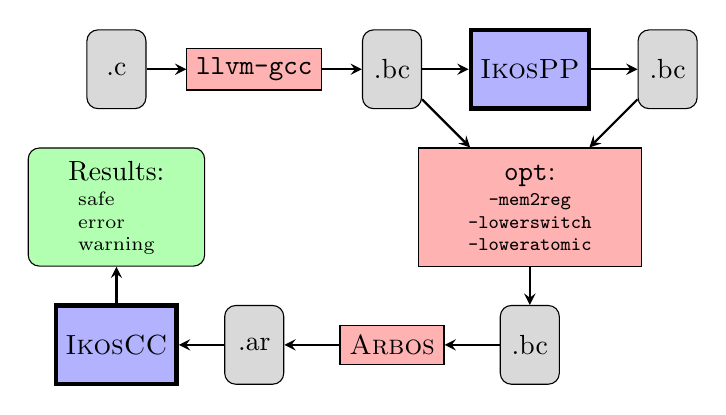
\begin{tikzpicture}[node distance=1.75cm]
%%%%%%%%%%%%%%%%
% nodes
%%%%%%%%%%%%%%%%
\node (c)  [file] {.c};
\node (llvmgcc) [tool, right of=c] {\llvmgcc};
\node (bc) [file, right of=llvmgcc] {.bc};
\node (ikospp) [ikoscc, right of=bc] {\ikospp};
\node (ppbc) [file, right of=ikospp] {.bc};
\node (opt) [tool, below of=ikospp] {
\begin{tabular}{c}
\llvmopt: \\
\begin{scriptsize}
%\setlength\tabcolsep{0}
\begin{tabular}{c}
\texttt{-mem2reg} \\
\texttt{-lowerswitch} \\
\texttt{-loweratomic}
\end{tabular}
\end{scriptsize}
\end{tabular}
};
\node (arbc) [file, below of=opt] {.bc};
\node (arbos) [tool, left of=arbc] {\arbos};
\node (ar) [file, left of=arbos] {.ar};
\node (ikoscc) [ikoscc, left of=ar] {\ikoscc};
\node (results) [results, above of=ikoscc] {
\begin{tabular}{c}
Results: \\
\begin{scriptsize}
\begin{tabular}{l}
safe \\
error \\
warning 
\end{tabular}
\end{scriptsize}
\end{tabular}
};
%%%%%%%%%%%%%%%%%
% arrows
%%%%%%%%%%%%%%%%%
\draw [arrow] (c) -- (llvmgcc);
\draw [arrow] (llvmgcc) -- (bc);
\draw [arrow] (bc) -- (ikospp);
\draw [arrow] (bc) -- (opt);
\draw [arrow] (ikospp) -- (ppbc);
\draw [arrow] (ppbc) -- (opt);
\draw [arrow] (opt) -- (arbc);
\draw [arrow] (arbc) -- (arbos);
\draw [arrow] (arbos)  --  (ar);
\draw [arrow] (ar) -- (ikoscc);
\draw [arrow] (ikoscc) -- (results);
\end{tikzpicture}
\end{minipage}
\end{center}
\caption{Architecture Overview}
\label{fig:architecture}
\end{figure}

Figure~\ref{fig:architecture} illustrates the overall architecture of
our static analyzer. 
%
First, a C input program is translated to LLVM bitcode~\cite{llvm} via
\llvmgcc.  Once we have obtained the bitcode, a pre-processor called
\ikospp performs optimizations and transformations. Such
pre-preprocessing is optional and its only mission is to optimize the
LLVM bitcode to make easier the task of static analysis. Even if the
pre-processor is disabled, we must use LLVM \llvmopt tool for
performing few transformations in order to ensure correct results: SSA
transformation, lowering of \texttt{switch} instructions into
\texttt{if-then-else}s, and lowering of \texttt{atomic} instructions.

Next, \arbos~\cite{ikos} translates the bitcode into an Abstract
Representation (AR) form. Before that, it performs some further LLVM
transformations such as ensuring the presence of only one exit block
per function, lowering constant expressions, and lowering
\texttt{select} instructions.  Compared to the LLVM bitcode, the AR
takes a different angle on how to express the semantics of a C
program.  
%
For example, $\phi$ nodes originated from SSA form are replaced with
assignments, the instruction set is more regular and the control flow
is expressed in a declarative way using non-deterministic choices and
\emph{assume}s rather than conditional branch instructions. Finally,
complex LLVM instructions such that \texttt{getElementPtr} used to
model pointer arithmetic are replaced by atomic operations on the
pointer offsets expressed in bytes.
%
The rationale behind the use of AR is that any generic abstract
interpretation algorithm can process it without any change in its
implementation.

Then, \ikoscc takes AR code as input, performs analysis on it, and
finally, reports the results to the user. Currently, results are being
stored in a database but it is straightforward to output the results
to different formats.
%
To facilitate the development of new analyses, \arbos provides a
\emph{plugin framework} that allows these analyses to use the AR code
as intermediate representation in a very simple way. This is very
similar to the functionality provided by the LLVM tool \texttt{opt}
but we replace the use of LLVM bitcode with AR code. All the analyses
implemented in \ikoscc are defined as \emph{arbos plugins}.

The rest of this document focuses on the two new components of our
architecture: \ikospp and \ikoscc. The rest of the components have
been described elsewhere (e.g.,~\cite{ikos}).

\section{\ikospp}
\label{sec:preprocessor}

\ikospp is a pre-processor that performs compiler optimizations and
pre-processing to simplify the static analysis task. %The use of
%\ikospp is completely optional and it does not affect the soundness of
%the results. 
The most relevant transformations are:

%% without bullets
%% As a first transformation we \emph{internalize} all functions to
%% enable global optimizations such as replacement of \emph{global
%%   aggregates} (e.g., arrays and structs) with \emph{scalars}. These
%% can have a huge impact later on the analysis since data that resides,
%% in principle, in the heap or stack can be lowered to registers and
%% therefore might be represented using integer variables. From the
%% perspective of a static analyzer, having a scalar variable facilitates
%% significantly the analysis' tasks since no memory reasoning is
%% needed. For instance, this code fragment: \texttt{struct foo $\{$ int
%%   x, int y $\}$; int main () $\{$ ... $\}$} might be transformed into:
%% \texttt{int main () $\{$ int x; int y;... $\}$}. We also perform dead
%% code elimination, and CFG simplifications to make the bitcode smaller
%% and simpler.  Some loop transformations are also performed to ensure
%% that loops have one single entry and exit, loop-closed SSA to satisfy
%% that no SSA variable is used outside of the loop, and simple
%% loop-invariant code motion.


\begin{itemize}

\item \emph{internalization} of all functions to enable global
  optimizations such as replacement of \emph{global aggregates} (e.g.,
  arrays and structs) with \emph{scalars}. These can have a huge
  impact later on the analysis since data that resides, in principle,
  in the heap or stack can be lowered to registers and therefore might
  be represented using integer variables. From the perspective of a
  static analyzer, having a scalar variable facilitates significantly
  the analysis' tasks since no memory reasoning is needed. For
  instance, this code fragment: 

\begin{small}
\begin{verbatim}
struct foo { int x; int y; }
int main () { ... }
\end{verbatim}
\end{small}

\noindent can be transformed into:

\begin{small}
\begin{verbatim}
int main () { int x; int y; }
\end{verbatim}
\end{small}

\item \emph{dead code elimination} and \emph{CFG simplifications} to
  make the bitcode smaller and simpler

\item some \emph{loop normalizations} to ensure that loops have one
  single entry and exit, \emph{loop-closed SSA} to satisfy that no SSA
  variable is used outside of the loop, and simple
  \emph{loop-invariant code motion}

%% \item \emph{removal of side-effect-free calls (e.g., printf-like
%%   calls)}. For instance, the removal of \texttt{printf} calls can
%%   trigger (via dead code elimination) the removal of strings in case
%%   they only feed these calls. Strings are represented in LLVM bitecode
%%   as constant global arrays of chars. 
\end{itemize}

Note that most of these transformations have often a direct impact
either in terms of accuracy (e.g., replacement of replacement of
aggregates into scalars) or efficiency (e.g., dead code
elimination). However, another major benefit from using \ikospp is the
possibility of replacing more expensive abstract domains with cheaper
ones without incurring in any loss of precision.
 

\begin{figure}[t]
  \centering
\begin{tabular}[h]{cc}
\begin{minipage}[t]{0.5\linewidth}
\begin{tabbing}
xx \= xx \= xx \= \kill
$\langle 1 \rangle$ \> \textbf{if} (*)  \\
$\langle 2 \rangle$ \> \> x = -10; \\
$\langle 3 \rangle$ \> \textbf{else}  \\
$\langle 4 \rangle$ \> \> x = 20; \\
$\langle 5 \rangle$ \> y=x; \\
$\langle 6 \rangle$ \> \textbf{if} (y $\leq$ 0) \\
$\langle 7 \rangle$ \> \> y = -x; \\
\end{tabbing}
\end{minipage} & 
\begin{minipage}[t]{0.5\linewidth}
\begin{tabbing}
xx \= xx \= xx \= \kill
$\langle 1 \rangle$ \> \textbf{if} (*)  \\
$\langle 2 \rangle$ \> \> x = -10; \\
$\langle 3 \rangle$ \> \textbf{else}  \\
$\langle 4 \rangle$ \> \> x = 20; \\
$\langle 5 \rangle$ \> \textbf{if} (x $\leq$ 0) \\
$\langle 6 \rangle$ \> \>   y = -x; \\
$\langle 7 \rangle$ \> \textbf{else} \\
$\langle 8 \rangle$ \> \>   y = x; \\
\end{tabbing}
\end{minipage} \\
\mbox{(a)} &  \mbox{(b)} \\
\end{tabular}
\caption{Original program and after transformed by \ikospp}
\label{fig:vmcai06-1}
\end{figure}


For example, if we would analyze the program in
Figure~\ref{fig:vmcai06-1}(a) with intervals~\cite{intervals} we would
infer before $\langle 5 \rangle$ is executed that $x \in [10,20]$ and
after $\langle 5 \rangle$ that $x \in [10,20],~ y \in [10,20]$. If
$\langle 7 \rangle$ is reached then we would have $y \in [-20,-10],
x\in [10,20]$ and after \emph{joining} with the else branch that keeps
unchanged $y$ we would obtain that $y \in [-20,20], x\in
[10,20]$. However, note that after $\langle 6 \rangle$ is executed we
know that $y$ cannot be a positive number but also the same for $x$
holds since we know that $x = y$. By adding this fact we could infer
after $\langle 7 \rangle$ that $y \in [0,10]$ and therefore after
joining with the omitted else branch we could have inferred a more
precise bound $y \in [-10,20]$.
%
Using a relational domain such as linear equalities~\cite{Karr76},
DBM\cite{dbm} or Octagons~\cite{octagons} we could have also inferred
the most precise bound for $y$. However, as we will describe in
Section~\ref{sec:analysis} these relational domains are more expensive
and we prefer to avoid them unless it is strictly necessary.
%
Min\'{e}~\cite{Minevmcai06} made first this observation and to mitigate
this problem he proposed a simple abstract domain to keep track of
syntactic relations~\cite{Minevmcai06} between variables that can be
combined with intervals while keeping same time complexity than
the original intervals.
%
Our main insight here is that \ikospp can help us avoid implementing
this new abstract domain since its transformations can cover some of
these cases. Figure~\ref{fig:vmcai06-1}(b) shows the transformed
program after executing \ikospp. Note that at line $\langle 5 \rangle$
\ikospp replaces $y$ with $x$ in the branch condition so that
intervals by itself can infer that $y \in [-10,20]$.


Although most of these transformations are provided directly by LLVM,
note that they focus on facilitating the task of code generation and
ultimately, reducing execution time and/or memory requirements. The
goal of \ikospp differs substantially from that since our goal is to
help static analysis by increasing precision and/or reducing analysis
time.

A good example of this mismatch is the LLVM pass \texttt{instcombine}
which performs peephole optimizations. Some of these optimizations
replace \texttt{mul X, 2} which is a linear arithmetic operation into
\texttt{shl X, 1} which is a bitwise operation. \todo{This is not 
  probably the best example.} For code generation the latter is better
because CPUs have generally specific instructions to perform left
shift in one clock cycle. However, thought most abstract domains can
model precisely linear arithmetic operations they cannot usually
handle bitwise operations and thus, we could have significant
precision losses. Another peephole optimization is to replace branch
instructions into logical operators. This can also have a very
negative impact on static analysis in terms of precision.\todo{Need to
  review this a bit. We ran some experiments and \texttt{instcombine}
  always improve our results.}
 
Another example is \texttt{indvars} which transforms each loop to have
a single canonical \emph{induction variable} starting at zero and
stepping by one. This transformation is very relevant because it can
trigger other LLVM optimizations that can further simplify or even
delete loops. It can help static analysis for at least two reasons:
speed up fixpoint convergence (most of the analyzer's time is spent on
loops), and it can improve the efficiency of relational domains since
within a loop only relations with respect to the induction variable
would suffice, and thus, it would reduce the need of keeping track
$O(n^{2})$ relations to $O(n)$. However, \texttt{indvars} rewrites
exit loop conditions which are inequalities (e.g., $x \leq 10$) into
disequations (e.g., $ x \neq 10 \equiv x < 10 \vee x > 10$). This can
produce significant precision losses since standard abstract domains
cannot reason about disjunctions.

Therefore, we also modify some of the steps performed by the above
LLVM passes to avoid incurring into unnecessary precision losses.

\ignore{
These issues can be avoided by disabling or modifying some of the
steps performed by the above LLVM passes. However, there are other
problems.

\begin{figure}[t]
  \centering
\begin{tabular}[h]{cc}
\begin{minipage}[t]{0.5\linewidth}
\begin{tabbing}
xx \= xx \= xx \= \kill
\textbf{int} x[10]; \\
\textbf{int} i; \\
\textbf{for} ($i=0$; $i < 10$; $i=i+1$) $\{$ \\
\> x[i] = 0; \\
$\}$ \\
\end{tabbing}
\end{minipage} & 
\begin{minipage}[t]{0.5\linewidth}
\begin{tabbing}
xx \= xx \= xx \= \kill
\textbf{int} x[10]; \\
\textbf{int} i, *b; \\
\textbf{for} (b = $\&$x[0]; ; $b=b+4$) $\{$ \\
\>   *b = 0; \\
\>   $i=i+1$; \\
\>   \textbf{if} ($i \geq 10$) \textbf{break}; \\
$\}$ \\
\end{tabbing}
\end{minipage} \\
\mbox{(a)} &  \mbox{(b)} \\
\end{tabular}
\caption{Original program and after induction variable transformation}
\label{fig:indvars}
\end{figure}


Figure~\ref{fig:indvars}(a) shows a program that traverses a C array
and updates each of its cells to zero, and Figure~\ref{fig:indvars}(b)
shows the same program after being transformed by
\texttt{-indvars}. For clarity, we show the corresponding C
transformed program rather than LLVM bitcode.

Let us assume that we would like to prove that the program in
Figure~\ref{fig:indvars}(a) cannot access the array \texttt{x} out of
bounds. For that, using intervals~\cite{intervals} we can infer that
$0 \leq i \leq 9$ inside the loop, and therefore all the array writes
are safe since the size of \texttt{x} is $10$. Using
Figure~\ref{fig:indvars}(b) we know that the induction variable is $i$
and we can still infer its bounds $0 \leq i \leq 9$ using
intervals. However, the array is now accessed via the pointer
\texttt{b}. In order to prove safety we need to infer the relationship
$b = 4 \times i$ (the constant $4$ is assuming the size of
\texttt{int} is $4$ bytes). This invariant cannot be expressed anymore
with intervals, and thus, we would need to use a more expressive (but
expensive) abstract domain. Note that even octagons are not expressive
enough. We would need to use at least TVPI~\cite{SimonK10}. With a
reduced product of intervals with congruences we would obtain $\langle
0 \leq i \leq 9, b \equiv 4\mathbb{Z} + 0\rangle$ but this does not
help.
}


%% // Another example from Mine's paper.
%% // Again, it turns out that LLVM optimizations is enough so no need of
%% // "linearization" here.
%% void lin_1(){
%%   int x,y,z;
%%   if (__ikos_unknown()) x= 5; else x=10;

%%   y = 3 * x - x; // LLVM ==> y = 2*x;

%%   __ikos_assert(y >= 10 && y <= 20);
%% }

%% // Another example from Mine's paper.
%% void lin_2(){
%%   int t,x,y,z;
%%   if (__ikos_unknown()) x= 5; else x=10;
%%   if (__ikos_unknown()) y= 2; else y=4;
%%   if (__ikos_unknown()) z= 6; else z=9;

%%   t = (x*y) - (x*z) + z;  // t = [-74,19]
%%   // LLVM ==> (y-z)*x +z ==> t = [-64,-1]
%%   __ikos_assert(t >= -74 && t <= 19);
%% }

\section{\ikoscc}
\label{sec:analysis}

This section assumes that the reader is familiar with the basic
concepts of Abstract Interpretation. Giving an introduction about
Abstract Interpretation is beyond the scope of this document. For
details, we refer to~\cite{Cousot_POPL77,CousotC79,NNH}.

Figure~\ref{fig:ikoscc} depicts the core of the analyzer.  First, the
AR code is translated into a standard Control Flow Graph (CFG). This
translation is straightforward since AR code already removed $\phi$
nodes (replaced with \emph{assignments}) and branch instructions
(replaced with \emph{assume}s), among other simplifications. Basic
blocks in the AR code are mapped to nodes in the CFG and edge $i
\rightarrow j$ is added in the CFG if a basic block $i$ is a
predecessor of block $j$ in the AR code.

At the core of all analyses we have a \emph{fixpoint iterator} and a
\emph{value analysis}. The fixpoint iterator computes the least fixed
point of a set of equations extracted from the semantics of the
program~\cite{intervals,Cousot_POPL77}. Since some domains might have
\emph{infinite ascending chains} termination must be ensured via a
\emph{widening} operator which is provided by the underlying abstract
domain. Moreover, a \emph{narrowing} operator must be also provided to
recover from precision losses caused by
widening~\cite{Cousot_PLILP92}. \ikoscc provides a state-of-the-art
fixpoint iterator that interleaves widening and narrowing in a very
precise manner~\cite{amatoSAS13}. However, other fixpoint iterators
can be plugin without effort. The semantics of the program is
approximated using a value analysis 'a la'
Min\'{e}~\cite{Mine06}. This value analysis computes for each program
variable the set of all possible values to which the variable can be
bound considering all possible executions.

Figure~\ref{fig:ikoscc} shows how the analyses interact with the
fixpoint iterator and the value analysis. All the analyses consist of
two phases: \emph{analysis} and \emph{check}. The goal of the analysis
phase is to compute all the invariants that hold at the entry of each
CFG node. To achieve this, a fixpoint over the CFG is computed. During
the fixpoint computation, given the abstract state $Pre^{\#}$ that
holds at the entry of a CFG node the value analysis computes its
abstract image $Post^{\#}$ representing the abstract state holding at
the exit of that node. Upon completion of the analysis phase, each
analysis checks for its property of interest using the invariants
computed during the analysis phase, and reports to the user the
results.

\begin{figure}[t]
\begin{center}
\begin{minipage}{1.0\linewidth}
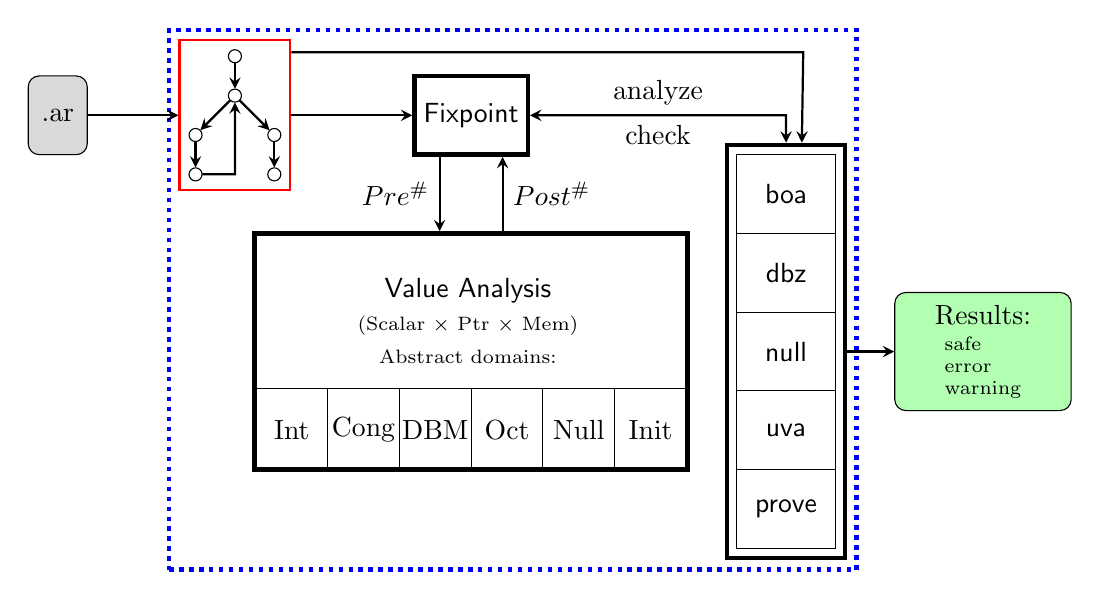
\begin{tikzpicture}
%%%%%%%%%%%%%%%%
% nodes
%%%%%%%%%%%%%%%%
\node (ar) [file,yshift=-2cm] {.ar};
%%
\node (entry) [stmt, scale=0.5,right of=ar,xshift=3.5cm,yshift=1.5cm] {};      
\node (loop) [stmt, scale=0.5,below of=entry] {};      
\node (looptt) [stmt, scale=0.5,left of=loop, below of=loop] {};      
\node (loopff) [stmt, scale=0.5,right of=loop, below of=loop] {};      
\node (loopbody) [stmt, scale=0.5,below of=looptt] {};      
\node (return) [stmt, scale=0.5, below of=loopff] {};      
\draw [edge,scale=0.5] (entry) -- (loop);
\draw [edge,scale=0.5] (loop) -- (looptt);
\draw [edge,scale=0.5] (loop) -- (loopff);
\draw [edge,scale=0.5] (looptt) -- (loopbody);
\draw[edge,scale=0.5] (loopbody.east) -- (4.5,-5.5) --  (loop);   
\draw [edge,scale=0.5] (loopff) -- (return);
%%
\node (cfg) [draw=red, thick, 
       fit={(entry) (loop) (looptt) (loopff) (loopbody) (return)}] {};

\node (fixpo) [fixpo, right of=entry, xshift=2cm,yshift=-0.75cm] {\textsf{Fixpoint}};
\node (va) [va, below of=fixpo, yshift=-2cm] {};
\node [below right, xshift=1cm] at (va.north west) {
  \begin{tabular}{c}
  \\
  \textsf{Value Analysis} \\
  \scriptsize (Scalar $\times$ Ptr $\times$ Mem) \\
  \scriptsize Abstract domains: 
  \end{tabular}
};
\DivRec{6}{1/Int,2/Cong,3/DBM,4/Oct,5/Null,6/Init}{domains}{va.south}

\node (boa) [analysis, right of=va,xshift=3cm,yshift=2cm] {\textsf{boa}};
\node (dbz) [analysis, below of=boa] {\textsf{dbz}};
\node (null) [analysis, below of =dbz] {\textsf{null}};
\node (uva) [analysis, below of=null] {\textsf{uva}};
\node (prover) [analysis, below of=uva] {\textsf{prove}};

\node (analyses) [draw=black, ultra thick, fit={ (boa) (dbz) (null) (uva) (prover)}] {};

\node (IkosCC) [draw=blue, ultra thick, dotted, fit={(cfg) (fixpo) (va) (analyses)}] {};
\node (results) [results, right of=analyses, xshift=1.5cm] {
\begin{tabular}{c}
Results: \\
\begin{scriptsize}
\begin{tabular}{l}
safe \\
error \\
warning 
\end{tabular}
\end{scriptsize}
\end{tabular}
};

%%%%%%%%%%%%%%%%%
% arrows
%%%%%%%%%%%%%%%%%
\draw [arrow] (ar) -- (cfg);
\draw [arrow] (cfg) -- (fixpo);
\draw [arrow] ([yshift=0.8cm] cfg.east) -- ++(6.5,0)  --  ([xshift=0.2cm] analyses.north);
\draw [arrow] ([xshift=-0.4cm]  fixpo.south)  --  ( [xshift=-0.4cm] va.north) node [midway, left] {$Pre^{\#}$};
\draw [arrow] ([xshift=0.4cm] va.north) -- ([xshift=0.4cm] fixpo.south) node [midway, right] {$Post^{\#}$};
\draw [arrow] (analyses) -- (results);
% \draw [arrow] (fixpo.east) --   (analyses.north);

\draw [arrow,<->] (fixpo.east)  -- node [left, above] {analyze} node [left, below] {check}  ++(3.25,0)  --  (analyses.north);

%\draw [arrow] ([yshift=0.1cm] va.east)  --  ([yshift=0.1cm] analyses.west) ;
%\draw [arrow] ([yshift=0.7cm] analyses.west) -- ([yshift=0.7cm] va.east);
\end{tikzpicture}
\end{minipage}
\end{center}
\caption{Internal Design of \ikoscc}
\label{fig:ikoscc}
\end{figure}

\subsection{Value Analysis}
\label{subsec:value}
%\vspace{2mm} 
%\noindent \textbf{Value Analysis.} 

We adopt the modular design of~\cite{Mine06} in which all the
operations performed by the value analysis are reduced to simpler
operations using a base numerical abstract domain. Here and in the
rest of this section, we refer to this base numerical abstract domain
as $\mathcal{N}^{\#}$. Similar to~\cite{Mine06} our value analysis can
also model program variables with different degrees of precision which
are presented from the coarsest to the finest:

\begin{enumerate}

\item integer scalars: models integer scalar variables originated
  from LLVM numeric \emph{registers}. Each of these scalar variables
  are mapped directly to a \emph{dimension} in $\mathcal{N}^{\#}$.
%This level of precision is suitable when only integer variables are
%relevant for the property of interest.

\item integer scalars and pointer addresses (but not contents): models
  integer and pointer registers. Each pointer $p$ represents a pair
  $\langle B, o \rangle$ where $B$ is the base address and $o$
  represents the offset from the base address of the object that
  contains $p$. A major benefit of using a low-level language like
  LLVM as input of our analyzer is that pairs $\langle B, o \rangle$
  are already represented as different pointer registers, and thus, in
  practice, each pointer register can be directly translated to a
  dimension in $\mathcal{N}^{\#}$.  For aliasing purposes, given a
  pointer $p$ we keep track, in a \emph{flow-sensitive} manner, of the
  set of possible memory locations ($\mathtt{\&}$'s addresses and
  \texttt{malloc}-like allocation sites) to which $p$ may point
  to. The points-to sets can also include function pointers. This
  level of precision is suitable when in addition to reason about
  integer scalars the analysis needs also to know if two pointers can
  point to the same memory location but it can ignore their contents.
  
\item memory contents: models integer scalars, pointer addresses, and
  pointer contents but only with integer type. The heap is modelled by
  a set of synthetic \emph{cells}. To deal precisely with pointer
  casts and type unions in C programs, a cell is represented by a
  triple $\langle B, i, s\rangle$ which models all the bits starting
  at offset $i$ starting from base address $B$ up to $i + s - 1$. As a
  result, each cell can then be mapped into another dimension in
  $\mathcal{N}^{\#}$. In this case, this new dimension approximates
  the content of the cell. For each memory read/write the value
  analysis needs to update accordingly these cells. In doing so,
  aliasing between cells must to be taken into account. This modelling
  is precise enough even in presence of pointer castings, pointer
  arithmetic, and function pointers.

  Note that a key feature of the Min\'{e}'s approach is that both
  integer scalars, pointer offsets, and cells are ultimately
  represented as dimensions in $\mathcal{N}^{\#}$. Nevertheless, this
  heap modelling is just an abstraction and therefore, we may lose
  precision in some cases. The main limitation is that cells can be
  only of integer type which means that we can only model pointers
  with one level of indirection. That is, we can model precisely the
  content of a pointer $p$ defined as $\texttt{int *p}$ but we cannot,
  for instance, to model the content of pointers of the form
  $\texttt{int **p}$.

\end{enumerate}

\subsection{Base Numerical Abstract Domains}

%\vspace{2mm}
%\noindent \textbf{Base Numerical Abstract Domains.} 

As we mentioned above, the value analysis reduces all its operations
to simpler operations using a base numerical abstract domain
$\mathcal{N}^{\#}$. New abstract domains can be easily added following
a very simple interface. Currently, \ikoscc provides out-of-the-box
the following classical domains:

\begin{itemize}

\item Int: intervals~\cite{intervals} expresses constraints of the
  form $\pm x \leq k$ where $ x$ is a variable and $k$ is a constant.

\item Cong: congruences~\cite{congruences} expresses constraints of
  the form $a\mathbb{Z} + b$ where $a$ and $b$ are integers. For
  instance, all even numbers are represented as $2\mathbb{Z} + 0$
  while all odd numbers are as $2\mathbb{Z} + 1$.

\item DBM: difference-bounds matrix~\cite{dbm} can express constraints
  $x - y \leq k$, where $x,y$ are variables and $k$ is a constant.

\item Oct: octagons~\cite{octagons} expresses constraints $\pm x \pm y
  \leq k$, where $x,y$ are variables and $k$ is a constant.

\end{itemize}

It is folklore in Abstract Interpretation that each of these domains
represents a trade-off between precision and complexity. The least
expensive domains are Int and Cong. Both have a time complexity of
$O(n)$ (where $n$ is the number of program variables). They are called
\emph{non-relational} domains because they model each variable alone
without considering the rest. Int is suitable for representing the
\emph{bounds} of a variable (e.g., the constraints $x \leq 100 \wedge
-x \leq -10$ denote that $x$ is between $10$ and $100$) while Cong can
model the \emph{density} of a variable by expressing for instance,
that $x$ is an even number or multiple of $6$ ($2\mathbb{Z} + 0$ and
$6\mathbb{Z} + 0$, respectively). DBM and Oct are called
\emph{relational} domains because they can express relations among
variables. For instance, the constraints $(x - y \leq 0)~ \wedge~ (y -
x \leq 0)$ denote that $x$ is equal to $y$ even if their bounds might
be unknown. DBM is strictly more precise than Int but its time
complexity increases to $O(n^{3})$. Oct is strictly more precise than
DBM and it preserves a worst-case time complexity of $O(n^{3})$. Cong
is incomparable to the other domains but usually too weak by
itself. For this reason, \ikoscc also implements a combination
(\emph{reduced product}) of Int with Cong (Int $\times$ Cong).

A key principle of the Abstract Interpretation framework is to build
complex abstract domains from the combination of simpler ones via
reduced product or functor domains. For this, \ikoscc provides support
for building reduced product of multiple abstract domains. For
instance, combinations of DBM or Oct with Cong or even better, reduced
products of DBM or Oct with Int $\times$ Cong can be implemented in a
straightforward manner.\footnote{Although DBM and octagons are
  strictly more expressive than intervals, non-linear operations such
  bitwise and logical operations can be still reasonably modelled
  using intervals but not using DBM or octagons. For this reason, it
  is often more recommendable to reduce first interval with
  congruences and then with DBM or octagons.}  \emph{Variable packing}
techniques (e.g.,~\cite{VenetB04,octagons,Bouaziz12}) are not
currently implemented.
%
%We have not implemented these cases since they have not been necessary
%for any of avionics programs analyzed so far. Similarly, for more
%expressive domains such as \emph{Two Variables per
%Inequality}~\cite{SimonK10} or \emph{Convex
%Polyhedra}~\cite{Cousot_Halbwachs_POPL78}.
More expressive relational domains such as \emph{Two Variables per
  Inequality}~\cite{SimonK10} or \emph{Convex
  Polyhedral}~\cite{Cousot_Halbwachs_POPL78} are also possible.

Finally, and for accuracy reasons, the value analysis also keeps track
of two important pieces of information: whether a pointer may be null
(Null) and whether a variable might be uninitialized (Init). The Null
domain models if a pointer is definitely null, definitely non-null or
otherwise, may be null. The Init domain models is a variable is
definitely initialized, definitely uninitialized or may be
initialized.

\subsection{Analyses}
 
%\vspace{2mm} \noindent \textbf{Analyses.} 

Once we have described all the main components we are ready to
describe in more details each of the analyses implemented in \ikoscc.

For each analysis the user can choose the base numerical abstract
domain as well as the level of precision. %% Our experimental evaluation
%% in Section~\ref{sec:results} shows the most suitable options for the
%% kind of applications we target here.
%
During the analysis phase, each analysis uses the same value analysis
and the only difference among them is during the check
phase. Therefore, each analysis keeps track of of the same numerical
invariants as well as nullity and uninitialized information. The
reason for this is that analyses such as \textsf{boa}, \textsf{dbz},
or \textsf{prove} can benefit from nullity information because it can
increase precision by detecting infeasible paths through reasoning
whether a pointer is null. On the other hand, \textsf{null} or
\textsf{uva} might benefit from numerical invariants because they can
also be more precise after detecting infeasible paths due to numerical
constraints.

Upon competition of the analysis phase we can assume that the value
analysis has computed the following functions ($\mathcal{V}$ is
the set of program variables):

\begin{itemize}

\item a function $R: \mathcal{V} \mapsto (\{-\infty \} \cup
  {\mathbb{Z}}) \times (\{+\infty \} \cup {\mathbb{Z}})$.
%
We use the notation $R(x) = [l,u]$ to represent that $l \leq x \leq
u$\footnote{Note that all the base domains implemented in \ikos pose
  an operation that converts from their representations to
  intervals. E.g., in the DBM abstract domain given the constraints $C
  \equiv x - y \leq 0 \wedge y -x \leq 0 \wedge y \leq 5 \wedge -y
  \leq -5$ the result of $R(x)$ can be computed by $\exists y. C
  \equiv x\leq 5 \wedge -x \leq -5 \equiv x = [5,5]$. Existential
  quantifier elimination is a common operation in abstract domains
  commonly named as \textsf{forget}.}. The symbol $\top$ represents
the interval $[-\infty, +\infty]$.

\item a function $I: \mathcal{V} \mapsto \{initialized, uninitialized,
  \top\}$, and

\item a function $N: \mathcal{V} \mapsto \{null, nonnull, \top\}$. 

\end{itemize}

\noindent The function $R$ maps each program variable to a range
(i.e., interval).  The function $I$ maps a program variable to whether
it is initialized or not, and the function $N$ maps a variable to
whether is null or not. The symbol $\top$ refers to a complete lack of
information. We describe next the main operations that each analysis
performs during the check phase.

\subsubsection{Buffer overflow (\textsf{boa})}

This analysis proves that there is no out-of-bounds array
accesses. That consists of checking each \texttt{load} or
\texttt{store} instruction that reads from or write to pointer $p$. In
that case, the value analysis has kept track of two variables $p_{o}$
and $p_{s}$ where

  \begin{itemize}
    
  \item $p_{o}$ is the offset from the base address of the object that
    contains $p$.
    
  \item $p_{s}$ is the actual size in bytes of the allocated memory
    for $p$ (including padding and alignment).
    
  \end{itemize}

\noindent Assume that $R(p_{s}) = [x,y]$ and the symbol $a \sqsubseteq
b$ returns true iff the interval $a$ is included in the interval $b$
(i.e., $ a \equiv [x_1,y_1] \sqsubseteq b \equiv [x_2,y_2]$ iff $x_1 \geq x_2$ and $y_1
\leq y_2$). Then, given a pointer $p$ we perform an \emph{overflow
  check}:

\begin{itemize}
\item if $R(p_{o}) \sqsubseteq [-\infty, y -1]$  then safe.
\item else if $R(p_{o}) \sqsubseteq [y, +\infty]$ then error.
\item otherwise, warning.
\end{itemize}

\noindent as well as an \emph{underflow check}:

\begin{itemize}

\item if $R(p_{o}) \sqsubseteq [0, +\infty]$ then safe.
\item else if $R(p_{o}) \sqsubseteq [-\infty, -1]$ then error.
\item otherwise, warning.
\end{itemize}

\noindent Therefore, note that an access to $p$ can be only considered
safe if both overflow and underflow conditions hold. That is,
$R(p_{o}) \sqsubseteq [-\infty, y -1]$ and $R(p_{o}) \sqsubseteq [0,
  +\infty]$ which is equivalent to say that $R(p_{o}) \sqsubseteq [0,
  y -1]$. The buffer overflow analysis also checks for memory
intrinsics such as \texttt{memcopy}, \texttt{memmove} and
\texttt{memset}.

%The default base numerical domain is Int $\times$ Cong. A minimum
%level of precision of \textsf{L2} (scalar and pointers) produces often
%a low warning rate but modelling of the heap (\textsf{L3}) produces
%even better results with a small overhead.

\subsubsection{Division by zero (\textsf{dbz})}

This analysis proves that there is no integer division by zero. For
each integer (signed or unsigned) division $x / y$ such that $R[y] =
[l,b]$:

\begin{itemize}
\item if $l=0$ and $u=0$ then error
\item else if $[0,0] \sqsubseteq [l,b]$ then warning
\item otherwise, safe.
\end{itemize}

%We have observed that after \ikospp simplifies the LLVM bitcode
%division operations require often very local reasoning and involving
%only integer scalars. Therefore, using Int with \textsf{L1} is usually
%enough.

\subsubsection{Null dereference (\textsf{null})}

This analysis proves that all the memory writes and reads cannot
de-reference a null pointer. For each memory access (i.e.,
\texttt{load} and \texttt{store}) through pointer $p$:

\begin{itemize}
\item if $N(p)$ is $nonnull$ then safe
\item else if $N(p)$ is $null$ then error
\item otherwise, warning
\end{itemize}

\subsubsection{Read uninitialized variables (\textsf{uva})}

This analysis proves that any used integer variable has been
previously initialized. For each used integer variable $v$:

\begin{itemize}
\item if $I(v)$ is $initialized$ then safe
\item else if $I(v)$ is $uninitialized$ then error
\item otherwise, warning

\end{itemize}

%% \item Prover of user-definable assertions (\textsf{prove}). To allow
%%   users to annotate the program with richer assertions we use a
%%   relational domain such as DBM with \textsf{L3}.


Common to all analyses a \emph{liveness analysis} is run as
pre-analysis step. The purpose is to infer which variables are
definitely \emph{dead} at the exit of each CFG node so we can
\emph{forget} those variables from $Post^{\#}$ before it is propagated
to the successor's $Pre^{\#}$. We observed that the impact on using
liveness information is mostly negligible for non-relational domains
but it can be very significant in the case of relational domains.

Finally, all the analyses can be used in an \emph{intra-procedural} or
\emph{inter-procedural} manner. In the former, each function is
analyzed ignoring its call context. In the latter, fully
context-sensitivity is achieved by inlining all program functions. We
have observed that inlining is a reasonable solution due to two main
reasons: (a) recursive functions are very rare in avionics software,
and (b) the exponential worst-case behavior has not been observed
after programs are pre-processed using \ikospp. %From the above
%analyses, only division by zero (\textsf{dbz}) is executed
%intra-procedurally.

\ignore{
\subsection{Implementation Details}
\label{subsec:implementation}

% efficient fixpoint based on WTO
% separate domain for non-relational domains
% finite domain implementation
}

\section{Usage}
\label{sec:usage}

Compiling multiple C files with LLVM requires modifying the Makefile
used to build the application so that the compiler tools invoked are
those provided by LLVM. This usually amounts to changing the settings
for the Makefile variables CC, LD and AR to \texttt{llvm-gcc},
\texttt{llvm-link}, and \texttt{llvm-ar}. It is very important to run
\texttt{llvm-gcc} with options \texttt{-c -emit-llvm} to generate LLVM
bitcode rather than binary executables.
%
Once we have obtained a single LLVM bitcode file, we provide a python
script to analyze the bitcode in a very simple way. The options for
running the analyzer are:

\begin{small}
\begin{verbatim}
ikos_cc [--cpu=CPU] [--mem=MEM] [--ikos-pp] INPUT -a ANALYSIS
\end{verbatim}
\end{small}

\noindent where \texttt{CPU} is the CPU time limit in seconds,
\texttt{MEM} is the memory limit in MB, \texttt{ikos-pp} runs \ikospp,
\texttt{INPUT} is a LLVM bitcode file (or alternatively, a C file),
and \texttt{ANALYSIS} is one of the following: boa, dbz, uva, prover,
and nullity. Upon termination, \ikoscc dumps all the checks into an
external database. The format of the checks is:

\begin{small}
\begin{verbatim}
name line number callstring status
\end{verbatim}
\end{small}

\noindent where \texttt{name} is a name for the check (e.g., buffer
overflow, buffer underflow, division by zero, etc), \texttt{line} and
\texttt{number} is the location of the check in the C file,
\texttt{callstring} is the call stack at the time of the check (empty
if intra-procedural analysis), and \texttt{status} is either:
\texttt{safe} (definitely safe), \texttt{unreachable} (definitely safe
because the check is dead code), \texttt{error} (definitely unsafe),
or \texttt{warning} (may be unsafe).
% 
Note that if the analysis is inter-procedural then it can have
multiple checks at the same \texttt{line} and \texttt{number} but with
a different \texttt{callstring}


\section{Experimental Evaluation}
\label{sec:results}

We have evaluated \ikoscc with several open-source autopilot control
software as well as software used in several NASA missions.
%
\textsf{paparazzi}~\cite{paparazzi} (20K LOC) and
\textsf{mnav}~\cite{mnav} (160K LOC) are both versatile autopilot
control software for a fixed-wing aircrafts and
multi-copters. \textsf{mnav} is fully implemented in C but
\textsf{paparazzi} is a mix of OCaml and C. For our experiments, we
only analyzed the C part. \textsf{gen2} (13K LOC) is automatically
code generated for several Simulink models\todo{Say which
  models?}. \textsf{SporeSat} is an autonomous, free-flying three unit
spacecraft. We analyzed one of its components\todo{We analyzed only
  the file \texttt{/1/sporesat2\_app\_spore}. Give description and
  size}. Neither the code for \textsf{gen2} or \textsf{SporeSat} is
publicly available.
%
All experiments have been carried out on an Red Hat Enterprise
Workstation machine with a 2.4 GHz AMD Opteron(TM) Processor 6136
and 8GB RAM.

%\floatsetup[figure]{style=plain,subcapbesideposition=top}
\begin{table}[tbh]
\begin{center}
  \subfloat[Modelling integer and pointer scalars using intervals with \ikospp]{
    \setlength{\tabcolsep}{1pt}
    \begin{tabular}{|l|c|c|c||c|c|c||c|c|c||c|c|c|}
      \hline 
      \textsf{Program} & \multicolumn{3}{|c||}{\textsc{boa}} & 
      \multicolumn{3}{|c||}{\textsc{uva}} &
      \multicolumn{3}{|c||}{\textsc{nul}} &
      \multicolumn{3}{|c|}{\textsc{dbz}} \\
      \hline 
      & $\mathsf{C}$ & $\mathsf{W}$ & $\mathsf{T}$ 
      & $\mathsf{C}$ & $\mathsf{W}$ & $\mathsf{T}$ 
      & $\mathsf{C}$ & $\mathsf{W}$ & $\mathsf{T}$  
      & $\mathsf{C}$ & $\mathsf{W}$ & $\mathsf{T}$  \\  
      \hline 
      \hline
      \textsf{paparazzi} & $908$  & $0$ & $24$ & $1181$ & $649$  & $25$ & $454$  & $0$ & $25$ & $3$ & $0$ & $6$  \\
      \hline
      \textsf{mnav}      & $5998$ & $2302$ & $59$ & $5860$ & $1232$ & $58$ & $2696$ & $895$ & $59$ & $1$ & $0$ & $6$  \\
      \hline
      \textsf{gen2}      & $10114$ & $264$ & $62$ & $1931$ & $420$ & $58$ & $5034$ & $51$ & $60$ & $2$ & $0$ & $14$  \\
      \hline
      \textsf{sporeSat}  & TBD & TBD & TBD &  TBD & TBD & TBD & TBD & TBD & TBD & TBD & TBD & TBD \\
      % TSS
      \hline 
    \end{tabular}
  } \\
  \subfloat[Modelling integer and pointer scalars and memory contents using intervals with \ikospp]{
    \setlength{\tabcolsep}{1pt}
    \begin{tabular}{|l|c|c|c||c|c|c||c|c|c||c|c|c|}
      \hline 
      \textsf{Program} & \multicolumn{3}{|c||}{\textsc{boa}} & 
      \multicolumn{3}{|c||}{\textsc{uva}} &
      \multicolumn{3}{|c||}{\textsc{nul}} &
                   \multicolumn{3}{|c|}{\textsc{dbz}} \\
                   \hline 
                   & $\mathsf{C}$ & $\mathsf{W}$ & $\mathsf{T}$ 
                   & $\mathsf{C}$ & $\mathsf{W}$ & $\mathsf{T}$ 
                   & $\mathsf{C}$ & $\mathsf{W}$ & $\mathsf{T}$  
                   & $\mathsf{C}$ & $\mathsf{W}$ & $\mathsf{T}$  \\  
                   \hline 
                  \hline 
                   \textsf{paparazzi} & $890$   & $0$  & $30$ &   $1152$ & $23$ & $30$ &  $445$ & $0$ & $30$     & \multicolumn{3}{c|}{} \\
\cline{1-10}
                   \textsf{mnav}      & $4730$  & $1343$ & $65$ & $4663$ & $838$ & $65$ &  $2169$ & $492$ & $65$ & \multicolumn{3}{c|}{} \\
\cline{1-10}
                   \textsf{gen2}      & $10114$ & $264$ & $73$ & $1931$ & $420$ & $73$ & $5034$ & $51$ & $73$ & \multicolumn{3}{c|}{} \\
\hline
                   \textsf{sporeSat}  & TBD & TBD & TBD  & TBD & TBD & TBD & TBD & TBD & TBD & TBD & TBD & TBD  \\
                   % TSS
                   \hline 
    \end{tabular}
  } \\
  \subfloat[Modelling integer and pointer scalars and memory contents using intervals without \ikospp]{
    \setlength{\tabcolsep}{1pt}
    \begin{tabular}{|l|c|c|c||c|c|c||c|c|c||c|c|c|}
      \hline 
      \textsf{Program} & \multicolumn{3}{|c||}{\textsc{boa}} & 
      \multicolumn{3}{|c||}{\textsc{uva}} &
      \multicolumn{3}{|c||}{\textsc{nul}} &
                   \multicolumn{3}{|c|}{\textsc{dbz}} \\
                   \hline 
                   & $\mathsf{C}$ & $\mathsf{W}$ & $\mathsf{T}$ 
                   & $\mathsf{C}$ & $\mathsf{W}$ & $\mathsf{T}$ 
                   & $\mathsf{C}$ & $\mathsf{W}$ & $\mathsf{T}$  
                   & $\mathsf{C}$ & $\mathsf{W}$ & $\mathsf{T}$  \\  
                   \hline 
\hline
                   \textsf{paparazzi} & $14890$ & $84$  & $12886$ & $2395$   & $107$ & $12795$ & $7417$ & $28$ & $12575$ & $25$ &$1$ &$85$ \\
\hline
                   \textsf{mnav}      & TBD &TBD &TBD &TBD &TBD &TBD &TBD &TBD &TBD &TBD &TBD &TBD \\
\hline
                   \textsf{gen2}      & TBD &TBD &TBD &TBD &TBD &TBD &TBD &TBD &TBD &TBD &TBD &TBD \\
\hline
                   \textsf{sporeSat}  & TBD &TBD &TBD &TBD &TBD &TBD &TBD &TBD &TBD &TBD &TBD &TBD \\
                   % TSS
                   \hline 
    \end{tabular}
  } 

\end{center}
\caption{\label{table:res}Analyses results on flight control software
  and NASA mission software}
\end{table}


Tables~\ref{table:res}(a)-(c) show the results of our evaluation. For each
program we ran the four analyses currently implemented in \ikoscc:
\textsc{boa} (buffer overflow analysis), \textsc{uva} (use of
uninitialized integer variable analysis), \textsc{nul} (null pointer
dereference analysis), and \textsc{dbz} (integer division by zero).
%
For each analysis we counted the total number of checks ($\mathsf{C}$),
the total number of warnings ($\mathsf{W}$), and the total time
($\mathsf{T}$) in seconds. \ikoscc did not find any definite error for
any of the programs and hence, we do not show that number.
%
For all experiments we always ran \textsc{boa}, \textsc{uva}, and
\textsc{null} in an inter-procedural manner and only \textsc{dbz} in
an intra-procedural manner. The reason is that unlike the other
analyses division by zero checks involve often very local reasoning
and hence, there is no need to run a much costly inter-procedural
analysis. 

Table~\ref{table:res}(a) shows the results of modelling integer and
pointer scalars using the interval domain and Table~\ref{table:res}(b)
shows the results of a similar configuration but modelling also
pointer contents. In both cases we ran \ikospp to optimize the LLVM
bitecode. Table~\ref{table:res}(c) uses the same configuration that
Table~\ref{table:res}(b) but after disabling the use of \ikospp. In
that way, we measure the effect of running the LLVM bitecode
pre-processor prior to any analysis.

First, \ikoscc was able to prove absence of integer division by zero
for \textsf{paparazzi}, \textsf{mnav}, and \textsf{gen2} as well
absence of buffer overflow and null pointer de-reference for
\textsf{paparazzi}. For other programs, such as \textsf{gen2}, the
number of warnings was very low for some analyses (e.g., \textsc{boa}
and \textsc{nul}) which allowed us to analyze it manually and
determine the main causes of those warnings (see
Section~\ref{sec:sec:warnings} for more details). \todo{Analysis of
  \textsf{sporeSat} is missing.}
%
Unlike for these programs, the results of \textsc{boa}, \textsc{nul},
and \textsc{uva} for \textsf{mnav} were less successful. We refer to
Section~\ref{sec:sec:warnings} for details.
%
The modelling of pointer contents (Table~\ref{table:res}(b)) shows
that it usually pays off in terms of precision with a reasonable
increase in analysis time. %% As expected, the precision gains are more
%% significant with analyses such as \textsc{uva} since there it is
%% crucial to model more precisely whether pointer contents are
%% initialized or not. For other analyses such as \textsc{boa} although
%% the modelling of pointers is also very important it might play a less
%% vital role since array indexes are less often stored in pointer
%% contents.
%
Finally, Table~\ref{table:res}(c) shows the dramatic impact of
\ikospp, described in Section~\ref{sec:preprocessor}, in terms of
precision as well as analysis time. The main reasons are that \ikospp
can lower many global C \texttt{struct}'s and variables to scalars,
reducing significantly the number of \emph{cells} that our value
domain needs to model. Similarly, \ikospp reduces significantly the
number of scalar variables which is also vital to keep the scalability
of the base numerical domains.

\textbf{TODO:} We should try with $Int \times Cong$. We will probably
get similar results. We would like to try with a relational domain,
such as DBMs, but currently we cannot since \emph{variable packing} is
not implemented and hence, DBMs run quickly out of resources.

\subsection{Causes of Warnings}
\label{sec:sec:warnings}

We have manually inspected some of our benchmarks and searching for
the possible causes of warnings returned by \ikoscc. We list here some
(but not all) of the reasons:

\begin{itemize}

\item In \textsf{gen2}, some numerical invariants are not expressible
  by \ikoscc abstract domains:

\begin{small}
\begin{verbatim}
  float*A, float*B; 
  for (i=0; i < 10; i++) 
    *p *= (*A++) * (*B++);
\end{verbatim}
\end{small}

\noindent For \textsc{boa}, we need to produce invariants $A_{o} = 4
\times i \wedge B_{o} = 4 \times i \wedge 0 \leq i \leq 9$ where
$A_{0}$ and $B_{0}$ are the offsets of $A$ and $B$, respectively, and
$4$ is the size of an integer in bytes. However, the invariants
required by $A_{o}$ or $B_{o}$ cannot be expressed with octagons, our
most expressive domain. For this kind of invariants we would need
TVPI~\cite{SimonK10} but it might be quite expensive. \todo{I think
  the Gauge domain~\cite{Gauge} would produce these invariants}

\item In \textsf{gen2}, current \ikoscc fixpoint iterator is not
  powerful enough with binary search-based lookups: \todo{This example
    is more complicated. There is an assumption that $\mathtt{x[bottom]}
    < u < \mathtt{x[top]}$ and also \texttt{u} is non-negative.}

\begin{small}
\begin{verbatim}
  bottom = some constant;
  top = some constant;
  for (;;) {
    idx = (bottom + top)/2;
    if (u <= x[idx])
      top = idx - 1;
    else if (u > x[idx+1]) 
      bottom = idx + 1;
    else {
      retValue = idx;
      break;
    }
  } 
\end{verbatim}
\end{small}

\noindent To prove that \texttt{x} cannot be accessed out of bounds we
need to infer that $\mathtt{bottom} \leq \mathtt{idx} \leq
\mathtt{top}$. However, note that $\mathtt{idx}$ is both incremented
and decremented in the loop. Therefore, widening will have effect on
both lower and upper bound of $\mathtt{idx}$ producing $-\infty \leq
\mathtt{idx} \leq \infty$. Narrowing does not improve the results.


\item In function \texttt{rtGetMinusInf} (\textsf{gen2}) floating
  point computation exploiting IEEE representation in the same spirit
  that the example in~\cite{Mine12}.\todo{Need to confirm this}

\item In \textsf{mnav}, the navigator component relies on a matrix
  library that creates matrices by allocating dynamic memory inside
  loops (\texttt{\_mat\_creat}):

\begin{small}
\begin{verbatim}
typedef struct {
   int	row;
   int	col;
}	MATHEAD;
typedef struct {
   MATHEAD	head;
   double	*matrix; // double
} MATBODY;
typedef   double	**MATRIX;// double
#define   Mathead(a) ((MATHEAD *)((MATHEAD *)(a) - 1))
#define   MatRow(a)	 (Mathead(a)->row)
#define   MatCol(a)	 (Mathead(a)->col)

MATRIX _mat_creat(int row, int col)
{
  MATBODY	*mat;
  int 	i;
  if ((mat = (MATBODY *)malloc( sizeof(MATHEAD) + sizeof(double *) * row)) == 0)
  { return NULL; };
  
  for (i=0; i<row; i++)
  {
    if ((*((double **)(&mat->matrix) + i) = (double *)malloc(sizeof(double) * col)) == 0)
    { return NULL); }
  }
  
  mat->head.row = row;
  mat->head.col = col;
  
  return (&(mat->matrix));
}
\end{verbatim}
\end{small}

\noindent Here, our value domain is not powerful enough to model
\texttt{malloc}'s inside loops. Nevertheless, the traversal of those
matrices (e.g., \texttt{mat\_copy}) is quite regular:

\begin{small}
\begin{verbatim}
MATRIX mat_copy(MATRIX A, MATRIX C)
{
  int i, j;
  for (i=0; i< MatRow(A); i++)
    for (j=0; j< MatCol(A); j++) {
      C[i][j] = A[i][j];
  }
  return(C);
}
\end{verbatim}
\end{small}

\noindent For \textsc{boa}, we would need the invariants for
\texttt{MatRow(A)} and \texttt{MatCol(A)} and the allocated size for
\texttt{A} and \texttt{B} but unfortunately we cannot infer any of
them.

\item \textsf{sporeSat} is significantly more complicated and
  different from standard avionics software we have seen so far. 
%
The global state is quite large. There many global arrays and
linked-lists that stores mutexes, message queues, etc. Memory
management is also more complicated than usual: there is a pool of
memory blocks which are already allocated. Each time there is a
request for a new memory block there is a loop that traverses all the
free memory blocks in the pool and returns the one with smallest size
that it is sufficient for the requested size \todo{This is just some
  of the problems. We need a much more detailed analysis}.

\end{itemize}

\ignore{
\section{Related Work}
\label{sec:related}

In a previous work, authors presented Ikos~\cite{ikos} a framework for
developing static analysis based on abstract interpretation. This
framework consists of two main components: \arbos to represent
succinctly CFGs from C programs and a library of fixpoint iterators
and abstract domains.
%
The work we propose here can be seen as an instantiation of this
framework. As a proof of concept, \cite{ikos} implemented only a
buffer overflow analysis and although its results on a set of avionics
benchmarks were impressive it did not modelled memory.

Therefore, the closest related work comes from more mature tools
relying on the abstract interpretation framework, namely C Global
Surveyor (\cgs~\cite{VenetB04}), CodeHawk~\cite{CodeHawk},
Astr\'{e}e~\cite{AstreeESOP05}, PolySpace Verifier~\cite{polyspace},
and Frama-C~\cite{frama-c}.

\astree focuses on safety-critical software while \ikoscc focuses on
on unmanned aerial flight control. %, on-board network management,etc?
Both \astree and \ikoscc implement the same value
analysis~\cite{Mine06} but \astree does not deal with
\texttt{malloc}'s at all while \ikoscc deals with arrays and
linked-lists to store pointers to semaphores, message queues, etc as
well as dynamically-allocated matrices that implement the logic of the
UAVs \todo{\ikoscc neither at this point but we would like to}. On the
other hand, \astree implements more sophisticated abstract domains
that allow modelling more precisely devices such as filters while
\ikoscc do not.

\cgs is very limited also with \texttt{malloc}s and it does not model
precisely dynamic memory inside loops. On the other hand, \cgs
implements a more compositional inter-procedural algorithm. \cgs uses
the reduced product of linear equalities~\cite{Karr76} with
intervals as the base numerical domain.

\textbf{TODO:}

\begin{itemize}

\item Similar to us, \framac relies on a value analysis based
  on~\cite{Mine06}. We should investigate if an experimental
  comparison is possible.

\item More recent abstract intepreters such as \textsc{Pagai}~\cite{pagai}:
a path-sensitive abstract interpreter based on SMT.

\end{itemize}
}

\section{Limitations and Future Extensions}
\label{sec:future}

Finally, we describe here some current limitations of the static
analyzer as well as some interesting future extensions.

At the level of front-end, our tool relies on unsupported legacy tools
(such as \texttt{llvm-gcc} and LLVM version 2.9), thus it is difficult
to maintain and extend. For instance, \texttt{llvm-2.9} cannot be
compiled with GNU compiler versions newer than \texttt{4.6} and there
is no \texttt{llvm-gcc} version for Windows machines. We would like to
replace \texttt{llvm-gcc} with
\texttt{clang}\footnote{\textbf{Author's note:} Historically, the
  reason of using \texttt{llvm-gcc} over \texttt{clang} has been that
  there is NASA software that cannot be compiled by \texttt{clang}. We
  need to review this claim because we tried with all the benchmarks
  we have and \texttt{clang} compiled all. \texttt{clang} is a very
  dynamic project so it has significantly improved over the years.}
which would also allow us replacing LLVM version 2.9 with a newer one
(e.g., version 3.6), or alternatively to use directly \texttt{gcc} via
\texttt{DragonEgg}~\cite{dragonegg}.

\vspace{2mm}
At the level of the analysis some of our current limitations are:

\begin{itemize}

\item all recursive calls are safely ignored.

\item inter-procedural analysis is done via inlining which might be
  prohibitive with large programs.

\item limited reasoning about dynamic memory allocation: \ikoscc does
  not distinguish between different instances of \texttt{malloc} in a
  loop. 

\item \ikoscc does not model pointer accesses with more than one level
  of indirection (e.g., \texttt{int **p; *p = q;} cannot be modelled
  precisely).

\item no reasoning about floating points (e.g.,~\cite{Mine12}): all
  floating point variables are safely ignored.

\item no machine arithmetic (e.g.,~\cite{Mine12,wrapped})

\end{itemize}

Note that not all of these analysis limitations have a real impact
when analyzing avionics software, and in fact, some of these absences
might have facilitated the design of our tool. For example, the use of
recursive call is a prohibited practice when implementing avionics
software. Therefore, it suffices for \ikoscc to analyze them in a
sound manner although imprecisely.

As a future work we plan to combine a \emph{position-sensitive}
pointer analysis (e.g.,~\cite{Venet04}) with our value analysis
presented in Section~\ref{sec:analysis}. This would allow us to reason
more precisely about dynamic memory allocation, in particular, with
deeper (i.e., multiple levels of indirection) memory accesses.
% and when we need to distinguish between different \texttt{malloc}
%instances in a loop.

We would like also to support \cpp. The design of a precise static
analyzer for \cpp is not trivial and it might require some re-design
in our tool. Our medium-term goal is to be able to analyze full \cpp
in a sound manner.

Finally, we would like to emphasize that \ikoscc has been carefully
crafted for being effective for certification of avionics software. It
has not been, however, designed for being a code style checker or
modelling syntax-oriented properties. Note that this is true even if
\ikospp is not used since LLVM bitcode lacks already of some
information such as signedness and some passes
(e.g.,\texttt{-mem2reg}) required before the translation to AR form
can apply already some transformations such as dead code
elimination. We also suggest to read the appendix in
Section~\ref{sec:undefined} for details about undefinedness in C
programs. To avoid all these issues, we would need to implement a new
tool at the front-end (e.g., \texttt{clang} or \llvmgcc) which is far
beyond the scope of this project.

\ignore{
\section{Conclusions}
TODO
}

\bibliographystyle{plain}
\bibliography{biblio}

\newpage 

\appendix 

\section{Notes about Undefined Behaviour in C}
\label{sec:undefined}

In this section, we recapitulate well-known consequences of undefined
behaviour in C programs and how they affect to the soundness of static
analyzers. 

In C programs, erroneous (buggy) operations such as null dereference,
or signed integer overflow are said to trigger \emph{undefined
  behaviour}. Although the presence of undefined behaviour indicates a
bug in the program, compilers are not forced to report an error or
even a warning. In fact, quoting the C FAQ compilers are completely
free to decide how to deal with undefined behaviour:


\begin{quote} 
\emph{Anything at all can happen; the Standard imposes no
  requirements. The program may fail to compile, or it may execute
  incorrectly (either crashing or silently generating incorrect
  results), or it may fortuitously do exactly what the programmer
  intended}.
\end{quote}

Although it might seem a bit surprising from the static analysis point
of view, the reason why the C Standard allows the existence of
undefined behaviour is to allow C being a very efficient low-level
programming language. 
%
For instance, \emph{use of uninitialized variables} is a common
example of undefined behaviour. This avoids compilers requiring all
variables must be zero initialized when they are in scope. This can
have a very positive impact on performance in presence of large stack
arrays and dynamically allocated memory. Another common example is
\emph{signed integer overflow}.  For instance, assuming that $\mathtt{INT\_MAX}
+ 1$ is undefined allows transforming $x + 1 > x$ into true. Note that
this simplification is not possible if we would assume that $\mathtt{INT\_MAX}
+ 1 = \mathtt{INT\_MIN}$. Another very important example is \emph{out of bounds
  array} accesses. The reason why out of bound accesses are left
undefined is that it avoids instrumenting programs with expensive
runtime checks ensuring that all accesses are in range. 


Therefore, it should be clear that the reason why undefined behaviour
exists is to allow compilers being smart and avoid dealing with
otherwise very costly situations. Similar rationale applies to other
cases such as \emph{division by zero}, \emph{null dereference},
\emph{oversized shift amounts} (shifting an 32 bit unsigned number by
32 bits or more), and \emph{violation of typing rules} (e.g., cast an
int* to float* and then dererefence it).

However, it should be obvious that compiler optimizations might have
negative effects on static analyzers that take as input compiler
optimized code rather than source code like in the case of
\ikoscc. These optimizations might hide bugs that \ikoscc will not be
able to find. In other words, \ikoscc can report a program to be safe
even if there is a bug.

To exemplify this phenomenon Figure~\ref{fig:undefined-ex} shows two
buggy programs that \ikoscc will report as safe.
%
The program in Figure~\ref{fig:undefined-ex}(a) has an use of an
uninitialized variable since $z$ is assigned to $5$ only if $argc$
is greater than $2$. Among others, \ikoscc executes the following
commands:
%
\begin{enumerate} 
\item \texttt{llvm-gcc test-1.c -c -emit-llvm -o test-1.bc} 
\item \texttt{opt test-1.bc -mem2reg -o test-1.pp.bc} 
\end{enumerate}
%
\noindent where command (1) is used to generate LLVM bitecode and (2)
is a requirement for \arbos. During the transformation
\texttt{mem2reg} the compiler notices that $z$ can be uninitialized
but instead of reporting an error or warning, it decides to
assign always $5$ to $z$ regardless the outcome of the comparison
$(argc > 2)$.

The program in Figure~\ref{fig:undefined-ex}(b) is buggy because the
assignment \texttt{a[i] = i} after the loop is writing in the array
$a$ at index $10$ but the array has been only allocated for indexes
between $0$ and $9$.
%
Perhaps, a bit surprising is that if we would execute the command
\texttt{llvm-gcc -O1 test-2.c -c -emit-llvm -o test-2.bc} we would see
that the program \texttt{test-2.bc} consists of one single statement
\texttt{return 0} so that \ikoscc claims the program to be trivially
safe since no checks are found. The reason for this is that the
compiler optimizations (triggered by flag \texttt{-O1}) can infer that
the loop is bounded and in fact, since the loop does not have any side
effects the compiler removes completely the loop. Moreover, the
compiler replaces the assignment \texttt{a[i] = i} with \texttt{a[10]
  = 10} and it realizes that the array write is out of bounds. Instead
of reporting an error or warning the compiler decides to remove the
array assignment.

We refer readers to~\cite{regehr-undefined,llvm-undefined} for more
examples and discussions describing how compiler optimizations can
make analysis tools unsound by taking advantage of the existence of
undefined behaviour in C programs.

\begin{figure}[t]
  \centering
\begin{tabular}[h]{cc}
\begin{minipage}[t]{0.5\linewidth}
\begin{tabbing}
xx \= xx \= xx \= \kill
int main (int argc, char **argv)  \\
$\{$ \\
\> int z, y; \\
\> \textbf{if} (argc > 2)  \\
\> \> z = 5; \\
\> \textbf{for} (y=0 ; y<5 ; y++) $\{$ \\
\> \> z = z + 1; \\
\> $\}$ \\
\> \textbf{return} z; \\
$\}$ 
\end{tabbing}
\end{minipage} & 
\begin{minipage}[t]{0.5\linewidth}
\begin{tabbing}
xx \= xx \= xx \= \kill
int main (int argc, char **argv)  \\
$\{$ \\
\> int i, a[10]; \\
\> \textbf{for} (i=0 ; i<10 ; i++) $\{$ \\
\> \> a[i] = i; \\
\> $\}$ \\
\> a[i] = i;\\
\> \textbf{return} 0; \\
$\}$ 
\end{tabbing}
\end{minipage} \\
\mbox{(a) \texttt{test-1.c}} &  \mbox{(b) \texttt{test-2.c}} \\
\end{tabular}
\caption{Examples of buggy programs that compilers can make them safe}
\label{fig:undefined-ex}
\end{figure}

The most obvious solution to this problem is to ensure that all
compiler optimizations are disabled. Considering our architecture
illustrated in Figure~\ref{fig:architecture} this would imply the
following steps:

\begin{enumerate}

\item Ensure that C programs are compiled by \llvmgcc without using
  any optimization (i.e., compilation flag \texttt{-O0}).

\item Disable all \llvmopt transformations described in
  Figure~\ref{fig:architecture} such as \texttt{mem2reg} and
  \texttt{lowerswitch}.

\item Disable the use of \ikospp.

\end{enumerate}

Step (1) might not be feasible in real situations. Avionics software
is usually deployed in very restricted environments in terms of
hardware resources. Therefore, it might be mandatory to highly
optimize (even \texttt{-O3}) the code before its deployment. Step (2)
is also hard to satisfy since these \llvmopt optimizations are
required to ensure the correctness of \arbos and hence, they cannot be
currently lifted. Finally, step (3) is the easiest to perform since
the use of \ikospp is optional. In this way, users can limit the
effect of compiler optimizations at the expense of longer analysis
time and less precise results as reported in
Section~\ref{sec:results}.
%

Therefore, unless we relax the requirements for \arbos and the
physical environment makes realistic to disable all compiler
optimizations \ikoscc users must account for the possibility that
compiler optimizations may hide bugs. However, based on our experience
the situation is not as bad as it might seem. Source code-based
analyzers\footnote{\llvmgcc provides, for instance, flags such as
  \texttt{Wuninitialized} to report users about uninitialized
  variables. We tried with \texttt{test-1.c} but we did not get any
  warning.}  can be used as a preliminary step before using
\ikoscc. This would allow to catch bugs that might be otherwise
eliminated by the compiler. Moreover, real avionics software does not
often contain so obvious examples like those illustrated in
Figure~\ref{fig:undefined-ex}. That is, bugs are often much more
subtle and compilers do not often encounter undefined behaviour in
this kind of applications.


\end{document}

